%
\documentclass[12pt]{article}

% The usual packages
\usepackage{fullpage}
\usepackage{breakcites}
\usepackage{setspace}
\usepackage{endnotes}
%\usepackage{float} % can't use with floatrow
\usepackage{amsmath}
\usepackage{amsfonts}
\usepackage{amssymb}
\usepackage{rotating}
\usepackage{longtable}
\usepackage{microtype}
\usepackage{graphicx}
\usepackage{hyperref}
%\usepackage[usenames,dvipsnames]{color}
\usepackage{url}
\usepackage{natbib}
\usepackage{framed} 
\usepackage{epigraph}
\usepackage{lipsum}
%\usepackage{dcolumn}
%\restylefloat{table}
\bibpunct{(}{)}{;}{a}{}{,}

% Set paragraph spacing the way I like
\parskip=0pt
\parindent=20pt

%\usepackage{helvet}
\usepackage[labelfont={bf}, margin=0cm, font=small, skip=0pt]{caption}


% Define mathematical results
\newtheorem{lemma}{Lemma}
\newtheorem{proposition}{Proposition}
\newtheorem{theorem}{Theorem}
\newtheorem{claim}{Claim}
\newenvironment{proof}[1][Proof]{\begin{trivlist}
\item[\hskip \labelsep {\bfseries #1}]}{\end{trivlist}}
\newenvironment{definition}[1][Definition]{\begin{trivlist}
\item[\hskip \labelsep {\bfseries #1}]}{\end{trivlist}}
\newenvironment{example}[1][Example]{\begin{trivlist}
\item[\hskip \labelsep {\bfseries #1}]}{\end{trivlist}}
\newenvironment{remark}[1][Remark]{\begin{trivlist}
\item[\hskip \labelsep {\bfseries #1}]}{\end{trivlist}}
\DeclareMathOperator*{\argmin}{arg\,min}
\DeclareMathOperator{\med}{med}
\DeclareMathOperator*{\E}{\text{E}}



%Set up fonts the way I like
\usepackage{tgpagella}
\usepackage[T1]{fontenc}
\usepackage[bitstream-charter]{mathdesign}

%% Baskervald
%\usepackage[lf]{Baskervaldx} % lining figures
%\usepackage[bigdelims,vvarbb]{newtxmath} % math italic letters from Nimbus Roman
%\usepackage[cal=boondoxo]{mathalfa} % mathcal from STIX, unslanted a bit
%\renewcommand*\oldstylenums[1]{\textosf{#1}}

%\usepackage[T1]{fontenc}
%\usepackage{newtxtext,newtxmath}

% A special command to create line break in table cells
\newcommand{\specialcell}[2][c]{%
 \begin{tabular}[#1]{@{}c@{}}#2\end{tabular}}


%% Set up lists the way I like
% Redefine the first level
\renewcommand{\theenumi}{\arabic{enumi}.}
\renewcommand{\labelenumi}{\theenumi}
% Redefine the second level
\renewcommand{\theenumii}{\alph{enumii}.}
\renewcommand{\labelenumii}{\theenumii}
% Redefine the third level
\renewcommand{\theenumiii}{\roman{enumiii}.}
\renewcommand{\labelenumiii}{\theenumiii}
% Redefine the fourth level
\renewcommand{\theenumiv}{\Alph{enumiv}.}
\renewcommand{\labelenumiv}{\theenumiv}
% Eliminate spacing around lists
\usepackage{enumitem}
\setlist{nolistsep}

% Create footnote command so that my name
% has an asterisk rather than a one.
\long\def\symbolfootnote[#1]#2{\begingroup%
\def\thefootnote{\fnsymbol{footnote}}\footnote[#1]{#2}\endgroup}

% Create the colors I want
\usepackage{color}
\definecolor{darkred}{RGB}{100,0,0}

\hypersetup{
pdftitle={Transformation-Induced Bias}, % title
pdfauthor={Carlisle Rainey}, % author
pdfkeywords={bias} {first difference} {marginal effect} {quantities of interest}
pdfnewwindow=true, % links in new window
colorlinks=true, % false: boxed links; true: colored links
linkcolor=darkred, % color of internal links
citecolor=black, % color of links to bibliography
filecolor=darkred, % color of file links
urlcolor=darkred % color of external links
}

% section headers
%\usepackage[scaled]{helvet}
%\renewcommand\familydefault{\sfdefault} 
%\usepackage[T1]{fontenc}
%\usepackage{titlesec}
%\titleformat{\section}
%  {\normalfont\sffamily\Large\bfseries}
%  {\thesection}{1em}{}
%\titleformat{\subsection}
%  {\normalfont\sffamily\large\bfseries}
%  {\thesection}{1em}{}
%  \titleformat{\subsubsection}
%  {\normalfont\sffamily\bfseries}
%  {\thesection}{1em}{}

% enable comments in pdf
\newcommand{\dtk}[1]{\textcolor{blue}{#1}}
\newcommand{\ctk}[1]{\textcolor{red}{#1}}


\begin{document}

\begin{center}
{\LARGE \textbf{Transformation-Induced Bias}}\\\vspace{2mm}
{ \textbf{Unbiased Coefficients Do Not Imply Unbiased Quantities of Interest}}\symbolfootnote[1]{All git computer code necessary for replication are available at \href{https://github.com/carlislerainey/transformation-induced-bais}{
github.com/carlislerainey/transformation-induced-bias}.}

\vspace{5mm}

Carlisle Rainey\symbolfootnote[3]{Carlisle Rainey is Assistant Professor of Political Science, University at Buffalo, SUNY, 520 Park Hall, Buffalo, NY 14260 (\href{mailto:rcrainey@buffalo.edu}{rcrainey@buffalo.edu}).}
\end{center}

\vspace{5mm}

% Abstract
{\centerline{\textbf{Abstract}}}
\begin{quote}\noindent
Political scientists commonly focus on quantities of interest computed from model coefficients rather than on the coefficients themselves. However, the quantities of interest, such as predicted probabilities, first differences, and marginal effects, do not inherit the small sample properties of the coefficient estimates. Indeed, unbiased coefficients estimates are neither necessary nor sufficient for unbiased estimates of the quantities of interest. I provide an approximation to the to this transformation-induced bias, illustrate its significance with two hypothetical examples, and highlight its importance to methodological research.
 \end{quote}

% Add quote to first page
% \epigraph{}

%\begin{center}
%Manuscript word count: 
%\end{center}

% Remove page number from first page
\thispagestyle{empty}

% Start main text
%\newpage
\doublespace

%\section*{Introduction}

Political scientists use a wide range of statistical models $y_i \sim f(\theta_i)$, where $i \in \{1,..., N\}$ and $f$ represents a probability distribution. The parameter $\theta_i$ is connected to a collection of covariates $X_i$ by an inverse link function $g$, so that $g(\theta_i) = X_i\beta$. The researcher can usually estimate $\beta$ with maximum likelihood (ML). Depending on the choice of $g$ and $f$, these estimates possess more or less desirable properties in small samples. For example, if the researcher correctly chooses the model $y_i \sim N(X_i\beta, \sigma^2)$, then the ML estimates of $\beta$ are unbiased. ML does not produce unbiased estimates in general, though, so studies developing new estimators frequently include Monte Carlo simulations to assessing the small sample properties and provide rules of thumb about appropriate sample sizes.

Although methodological research tends to focus on estimating the model coefficients, the coefficients themselves are often of indirect interest to substantive researchers. Instead, substantive researchers tend to focus on a a \textit{transformation} $\tau$ of the model coefficients or a ``quantity of interest'' \citep{KingTomzWittenberg2000}. Examples include marginal effects, first and second differences, predicted probabilities, and expected counts. Fortunately, it is straightforward to transform ML estimates using the invariance property, which states that if $\hat{\theta}$ is the ML estimate of $\theta$, then for any function $\tau$, the ML estimate of $\tau(\beta)$ is $\tau(\hat{\theta})$ (\citealt[pp. 75-76]{King1989}, and \citealt[pp. 320-321]{CasellaBerger2002}). %King (1998, p. 75-76) writes: 
%\begin{quote}
%Often researchers prefer to estimate a function of a parameter rather than a parameter itself. The invariance property of ML estimators guarantees that one can estimate either and transform them as needed.
%\end{quote}
Of course, if $\hat{\theta}$ is a consistent estimator of $\theta$, then $\tau(\theta)$ is a consistent estimator $\tau(\hat{\theta})$. But the invariance principle raises an important question: Does $\tau(\hat{\theta})$ necessarily inherit desirable small sample properties of $\hat{\theta}$, such as unbiasedness? The answer is no. Under the assumption the linear model and iid normal errors, least squares estimates have excellent small sample properties (i.e., best unbiased estimator), but quantities of interest calculated from these unbiased coefficient estimates might be strongly biased.

The point is crucial--it connects the work done by methodologists, which tends to focus on coefficients, to the work done by substantive scholars, which tends to focus on a transformations of the coefficients. Much (though certainly not all) methodological research that we do implicitly suggests that an approximately unbiased coefficient estimate is necessary and/or sufficient for an approximately unbiased estimate of the quantity of interest. Classically, \cite{Nagler1994} uses Monte Carlo simulations to assess the small sample properties of the scobit model coefficients but focuses on marginal effects and predicted probabilities in his illustrative application. Recently, \cite{Nieman2015} uses simulations to assess the small sample properties of the coefficients in his strategic probit with partial observability, but focuses his illustrative application on predicted probability of civil war. In order to provide more compelling tools for substantive scholars, we must extend their focus beyond coefficients to quantities of interest.

\subsection*{The Concepts}

As a motivating example, consider the log-linear model 
\begin{equation}
\log (\text{income}_i) = \beta_{cons} + \beta_{edu} \text{education}_i + \epsilon_i \text{,}\nonumber
\end{equation}
where $\epsilon_i \sim N(0, \sigma^2)$ and we suppose that education is measured in years and income in thousands of dollars. Assuming that we have the correct model, then least squares (which corresponds to the ML estimator) provides the best unbiased estimator of the model parameters $\beta_{cons}$ and $\beta_{edu}$. However, we are not likely interested in $\log(\text{income})$ directly. Instead, we are likely interested in income itself. Suppose that we are interested in the quantity $\med(\text{income} | \text{education} = 20) = e^{\beta_{cons} + 20\beta_{edu}}$. One might erroneously infer that unbiased estimates of $\beta_{cons}$ and $\beta_{edu}$ lead to unbiased estimates of $\med(\text{income} | \text{education} = 20)$, but that is not the case. If we suppose that $N = 10$, $\beta_{cons} = 2.5$, $\beta_{edu} = 0.1$, $\sigma^2 = 1$, and \textit{education} takes on integers roughly uniformly from 10 to 20, then $\tau(\beta_{cons}, \beta_{edu}) = e^{\beta_{cons} + 20\beta_{edu}} \approx \$90k$. To calculate the bias in the quantity of interest, I simulate 100,000 data sets and calculate the quantity of interest for each. Although $\hat{\beta}_{cons}$ and $\hat{\beta}_{edu}$ are unbiased, $\med(\text{income} | \text{education} = 20)$ is strongly biased upward, with an expected value of about $\$106k$.

We usually think about bias as occurring in the model coefficients $\beta$, so that 
\begin{equation}
\text{coefficient bias} = \E(\hat{\beta}) - \beta \text{.}  \nonumber
\end{equation}
But substantive researchers care mostly about bias in the quantities of interest, which I refer to as $\tau$-bias, so that
\begin{equation}
\tau\text{-bias} = \E[\tau(\hat{\beta})] - \tau(\beta)\text{.} \nonumber
\end{equation}
$\tau$-bias is more complex and subtle than biases in the coefficients. It can be rewritten and decomposed into two components: transformation-induced $\tau$-bias and coefficient-induced $\tau$-bias, so that
\begin{equation}
\tau\text{-bias}= \underbrace{ \E[\tau(\hat{\beta})]-  \tau[\E(\hat{\beta})]  }_{\text{transformation-induced}} + \overbrace{  \tau[\E(\hat{\beta})] - \tau(\beta)  }^{\text{coefficient-induced}}\text{.} \nonumber
\end{equation}
Any coefficient bias passes through to the quantities of interest in the sense that transformation of the average coefficient is not equal to the transformation of the true coefficient.
\begin{equation}
\text{coefficient-induced } \tau\text{-bias} = \tau[\E(\hat{\beta})] - \tau(\beta) \nonumber
\end{equation}
Because $g[\E(X)] \neq \E[g(X)]$ in general, the transformation itself introduces bias as well. 
\begin{equation}
\text{transformation-induced } \tau\text{-bias} = \E[\tau(\hat{\beta})]-  \tau[\E(\hat{\beta})] \nonumber
\end{equation}
Methodologists do not often explicitly recognize this transformation-induced $\tau$-bias and few seem to fully appreciate its importance. Below I offer a general characterization using Jensen's inequality, and approximation to its magnitude, and two examples that illustrates its significance.

%While it is possible that the two components of $\tau$-bias cancel each other, it is also possible that the two compound each other. 

\subsection*{A Characterization}

Jensen's inequality allows straightforward characterization of the direction of the transformation-induced $\tau$ bias for strictly convex or strictly concave transformations. It also provides the key intuition for more complicated transformations and the approximation below.

\begin{theorem}
Suppose a generic (non-degenerate) ML estimator $\hat{\beta}$. Then any strictly convex (concave) $\tau$ creates upward (downward) transformation-induced $\tau$-bias.
\end{theorem} 
\begin{proof}
The proof follows directly from Jensen's inequality. Simply suppose that the non-degenerate sampling distribution of $\hat{\beta}$ is given by $S_\beta(b)$. Then $\E[\hat{\beta})] = \int_{B}bS_\beta(b)db$ and $\E[\tau(\hat{\beta})]  = \int_{B}\tau(b)S_\beta(b)db$. Suppose first that $\tau$ is convex. By Jensen's inequality, $\int_{B}\tau(b)S_\beta(b)db > \tau \left[ \int_{B}bS_\beta(b)db \right]$, which implies that $\E[\tau(\hat{\beta})] > \tau[\E(\hat{\beta})]$. Thus, $\E[\tau(\hat{\beta})] - \tau[\E(\hat{\beta})] > 0$. By similar argument, one can show that for any strictly \textit{concave} $\tau$, $\E[\tau(\hat{\beta})] - \tau[\E(\hat{\beta})] > 0$.
\end{proof}

In general, researchers do not restrict themselves to a strictly convex or strictly concave $\tau$. For example, quantities from logistic regression models, such as predicted probabilities, first and second differences, and marginal effects all convex regions and concave regions. This situation is much more difficult to characterize generically, given that $\tau(b)$ might contain a mixture of strictly convex and strictly concave regions or at any particular point $b$, the multivariate function $\tau$ might be convex in one direction and concave in another. In general though, the direction of the bias depends on the \textit{location} of the sampling distribution. If most of the sampling distribution is located in a ``mostly concave'' region, then the bias will be downward. If most of the sampling distribution is located in a ``mostly convex'' region, then the bias will be upward. 

\subsection*{An Approximation}

Next, I approximate the magnitude of the the transformation-induced $\tau$-bias using a second-order Taylor expansion. First, notice that $\E[\tau(\hat{\beta})] = \E[\tau(\E[\hat{\beta}] + (\hat{\beta} - \E[\hat{\beta}]))]$. Now approximate the term inside the right-hand expectation with a second order Taylor expansion, so that 
\begin{equation}
E[\tau(\hat{\beta})] \approx \E \left[ \tau[\E(\hat{\beta})] + \displaystyle \sum_{r = 1}^k \dfrac{\partial \tau(\beta)}{\partial \beta_r}[\hat{\beta}_r - \E(\hat{\beta}_r)] +  \dfrac{1}{2} \displaystyle \sum_{r = 1}^k \sum_{s = 1}^k \dfrac{\partial^2 \tau(\beta)}{\partial \beta_r \beta_s}[\hat{\beta}_r - \E(\hat{\beta}_r)][\hat{\beta}_s - \E(\hat{\beta}_s)] \right ]\nonumber
%\E[\tau(\hat{\beta})] & \approx \E[\tau(\beta)]  + \dfrac{1}{2} \displaystyle \sum_{r = 1}^k \sum_{s = 1}^k H_{rs} \Sigma_{rs}\text{,} \no number
\end{equation}
Taking the expectation of the right-hand side eliminates the middle term and allows expressing the final term as a function of the variance of the sampling distribution, so that 
\begin{equation}
\E[\tau(\hat{\beta})] \approx  \tau[\E(\hat{\beta})]  + \dfrac{1}{2} \displaystyle \sum_{r = 1}^k \sum_{s = 1}^k H_{rs}(\beta) \Sigma_{rs}\text{,} \nonumber
\end{equation}
where $H(\beta)$ represents the Hessian matrix of second derivatives of $\tau$ at the point $\beta$ and, conveniently, $\Sigma$ represents the (co)variance matrix of the sampling distribution. Rearranging gives an approximation to the magnitude of the transformation-induced $\tau$-bias, so that 
\begin{equation}\label{eqn:bias}
\text{transformation-induced } \tau\text{-bias} = \E[\tau(\hat{\beta})] - \tau[\E(\hat{\beta})]  \approx \dfrac{1}{2} \displaystyle \sum_{r = 1}^k \sum_{s = 1}^k H_{rs}(\beta) \Sigma_{rs}\text{.} \nonumber
\end{equation}
If $H$ is constant then the approximation is exact. 

Equation \ref{eqn:bias} does not depend on a strictly convex or concave transformation. The approximation is reasonable if $H(\beta)$ resembles the curvature of $\tau$ over most of the sampling distribution. As long as $\tau$ is not highly non-linear (e.g., $\left|\frac{\partial^3 \tau}{\partial \beta_r \partial \beta_r\partial \beta_rs \partial \beta_t}\right| >> 0$), then Equation \ref{eqn:bias} provides a reasonable estimate of the direction and magnitude of the bias.

Equation \ref{eqn:bias} quantifies two intuitions. First, the amount of bias depends on the standard error and/or sample size. As the sample size grows large, $\Sigma$ shrinks to zero along with the bias. This observation matches the fact that $\tau(\hat{\beta})$ is a consistent estimator of $\tau(\beta)$. Secondly, the amount of bias depends on the curvature in $\tau$. If $\tau$ is nearly linear, then the transformation introduces minimal bias. More curvature, on the other hand, leads to greater bias. 

\subsection*{An Example}

Many substantive researchers realize that logistic regression estimates are biased away from zero in small samples. However, fewer realize that a simple penalized applied to the likelihood function can nearly eliminate this bias \citep{Firth1993}. In this example, I show Firth's effort in obtaining unbiased coefficients can be lost if researchers focus on marginal effects.

For concreteness, suppose a model explaining the probability of voting as a function of education
\begin{equation}
\Pr (\text{vote}_i) = \text{logit}^{-1(}\beta_{cons} + \beta_{edu} \text{education}_i) \text{,}\nonumber
\end{equation}
where \textit{vote} indicates whether or not citizen $i$ voted in the election and \textit{education} is measured in years. Let $\beta_{cons} = -2.5$, $\beta_{edu} = 0.2$, and $N = 30$. Assume we are interested in the marginal effect of education. In this case, we have might want to calculate the marginal effect of education at a substantively relevant value (e.g., \textit{education} = 12 years or \textit{education} = 16 years), at all observed values, or perhaps average across all the observed data \citep{HanmerKalkan2013}.

I first create a hypothetical variable \textit{education} that takes on 30 integer values roughly uniformly distributed from 10 to 20. I then simulate 100,000 data sets and compute the coefficients and marginal effects for each data set using ML and penalized ML estimation. As expected, the ML coefficient estimates (intercept and slope) are biased away from zero by about 14\% and the penalized ML estimates are biased about 1\%.

But compare the sampling distribution for the quantity of interest $\tau$ calculated using the strongly biased ML estimate $\hat{\beta}^{mle}$ and the essentially unbiased penalized ML estimate $\hat{\beta}^{pmle}$. At first glance, one might guess that the $\tau(\hat{\beta}^{pmle})$ would provide a less biased estimate of $\tau(\beta)$. However, that does not follow. A \textit{more biased} estimate of $\beta$ might lead to a less biased estimate of $\tau(\beta)$ if the two coefficient- and transformation-induced $\tau$-bias cancel. This is exactly what happens in the hypothetical example. Figure \ref{fig:logit-me-bias} shows that the estimate of the marginal effect of education on the probability of voting is consistently biased downward when calculated from the nearly unbiased $\hat{\beta}^{pmle}$. This downward bias is true for all values of education. On the other hand, marginal effects calculated using the biased coefficient estimate $\hat{\beta}^{mle}$ are sometimes biased downward, sometimes upward, and other times little. Of the 11 `possible values of education in the hypothetical data set (10 to 20 years), the biased ML estimate leads to less biased marginal effects in six cases. The nearly unbiased penalized ML estimates lead to less biased marginal effects in only four cases. (The remaining case is essentially a tie.)

\begin{figure}[h!]
\begin{center}
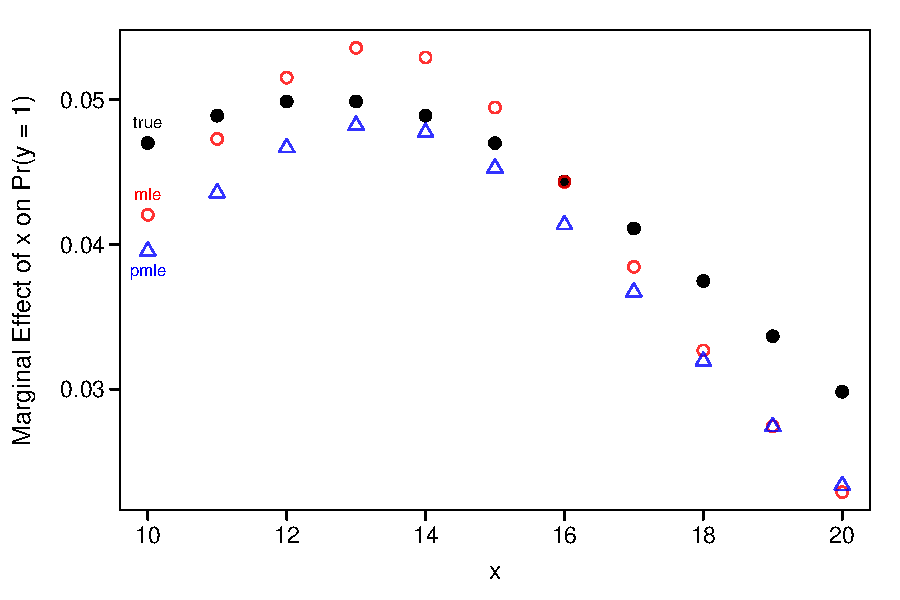
\includegraphics[scale = 0.7]{figs/logit-me-bias.pdf}
\caption{This shows the true marginal effects and the expected values of the ML and penalized ML estimates of the marginal effects. Although the ML coefficient estimates are strongly biased away from zero, these coefficient estimates provide less biased estimates of the marginal effects for more than half of the observed values of $x$. While the penalized ML estimates of the coefficients are essentially unbiased, these estimates provide less biased estimates of the marginal effects in only three of the eleven cases and \textit{always} underestimate the marginal effects.}\label{fig:logit-me-bias}
\end{center}
\end{figure}

Notice that if we focused on the marginal effect at \textit{education} = 12 or \textit{education} = 16, then the biased ML coefficient estimate provides a less biased estimate of the marginal effect. If we average across the marginal effects at the for the observed data, following \cite{HanmerKalkan2013}, the essentially unbiased penalized ML coefficient estimates have a downward bias of about 10\%. The strongly biased ML coefficient estimates, on the other hand, have a downward bias of only about 2\%.

\subsection*{The Implications}

The general fact that $\E[\tau(\hat\beta)] \neq \tau[\E(\hat\beta)]$ has important implications for how we study the small sample properties of estimators. In practice, methodologists usually parameterize estimators so that $\beta_r$ lies in the real line. This allows the estimator $\hat{\beta}$ to rapidly approach its asymptotic distribution, which ensures $\hat{\beta}$ has acceptable small sample properties. Substantive researchers, though, usually transform these coefficients into quantities of interest $\tau(\hat{\beta})$, and the estimated quantity of interest does not inherit the small sample properties of the coefficient estimators. Because the quantity of interest often lies in a bounded space, such as $[0, 1]$ or $(0, \infty)$, it might approach its asymptotic distribution more slowly. As a result, approximately unbiased estimates of quantities of interest might require much larger sample sizes than studies of coefficients recommend.

Secondly, there is usually a tradeoff between bias and variance in estimating parameters. However, the approximation to the transformation induced bias given in Equation \ref{eqn:bias} points out an important fact. Greater variance in the coefficient estimates lead to increased bias in the quantities of interest. This implies that if an estimator is essentially unbiased, then greater efficiency translates to reduced bias in the quantities of interest. Similarly, small reductions in bias at the expense of large loss in efficiency might lead to greater bias in the quantities of interest. 

As methodologists, we cannot ignore transformation induced bias. Essentially unbiased estimators of coefficients are not enough. We must be aware of the quantities of interest to substantive researchers and calibrate our tools for these quantities.

\singlespace 
%\newpage
\small
\bibliographystyle{apsr_fs}
\bibliography{/Users/carlislerainey/Dropbox/papers/bibliography/bibliography.bib}

\end{document}


















